% "Why theta-hat converges at rate 1/sqrt(m)" — a standalone explainer deck
% Decodes the Section-4 claim theta-hat = theta* + O_p(m^{-1/2}) and Appendix B
% of Nagler '23 (Statistical Foundations of PFNs).
% Self-contained: no external images. Build with:  make   (tectonic)
\documentclass[aspectratio=169,10pt]{beamer}

\usetheme{metropolis}
\metroset{progressbar=frametitle, numbering=fraction, block=fill}

\usepackage{booktabs}
\usepackage{amsmath,amssymb}
\usepackage{tikz}
\usetikzlibrary{positioning,arrows.meta,fit,backgrounds,calc,decorations.pathreplacing}
\usepackage{pgfplots}
\pgfplotsset{compat=1.18}
\usepackage{xcolor}

% --- palette (matches the main talk) ---------------------------------------
\definecolor{accent}{HTML}{C1121F}
\definecolor{ink}{HTML}{2B2D42}
\definecolor{muted}{HTML}{6C757D}
\definecolor{good}{HTML}{2A9D8F}
\setbeamercolor{frametitle}{bg=ink}
\setbeamercolor{background canvas}{bg=white}
\setbeamercolor{normal text}{fg=ink, bg=white}
\setbeamercolor{progress bar}{fg=accent}
\setbeamercolor{alerted text}{fg=accent}

\newcommand{\hl}[1]{{\color{accent}\textbf{#1}}}
\newcommand{\gd}[1]{{\color{good}\textbf{#1}}}
\newcommand{\mut}[1]{{\color{muted}#1}}
\newcommand{\cit}[1]{{\scriptsize\color{muted}[#1]}}

\title{Why pre-training converges at rate $1/\sqrt{m}$}
\subtitle{The Section 4 claim $\hat\theta=\theta^*+O_p(m^{-1/2})$ --- and Appendix B \cit{Nagler '23}}
\author{\underline{Gurmeher} Singh Puri}
\institute{Explainer deck --- the PFN approximation result}
\date{}

\begin{document}

\maketitle

% ===========================================================================
\begin{frame}[t]{First: $m$ is \emph{not} the famous size}

  \onslide<1->{\centering Section 4 has \hl{two different ``sizes''} --- don't conflate them in Q\&A.\par}
  \vspace{0.7em}

  \begin{columns}[T]
    \column{0.5\textwidth}
      \onslide<1->{\centering \textbf{Pre-training} \;\mut{(offline)}\\[5pt]
      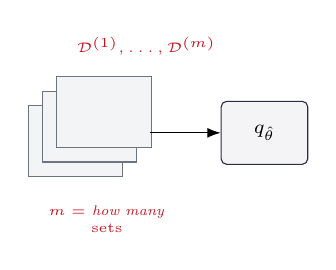
\begin{tikzpicture}[>=Latex, font=\scriptsize]
        % a stack of m datasets
        \foreach \i in {0,1,2} {
          \draw[muted, fill=muted!8, line width=0.4pt]
            ({\i*0.18},{\i*0.18}) rectangle ({\i*0.18+1.2},{\i*0.18+0.9});
        }
        \node[align=center, font=\tiny, text=accent] at (1.5,1.65) {$\mathcal{D}^{(1)},\dots,\mathcal{D}^{(m)}$};
        \node[draw=ink, fill=ink!5, rounded corners=2pt, minimum width=11mm, minimum height=8mm]
              (q) at (3.0,0.55) {$q_{\hat\theta}$};
        \draw[->] (1.55,0.55) -- (q);
        \node[font=\tiny, text=accent, align=center] at (1.0,-0.55) {$m=$ \emph{how many}\\ sets};
      \end{tikzpicture}}
    \column{0.5\textwidth}
      \onslide<2->{\centering \textbf{Inference} \;\mut{(one forward pass)}\\[5pt]
      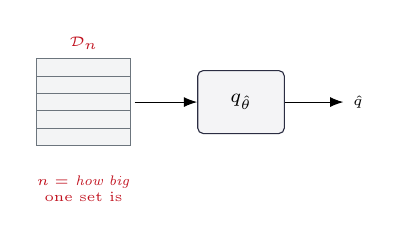
\begin{tikzpicture}[>=Latex, font=\scriptsize]
        \draw[muted, fill=muted!8, line width=0.4pt] (0,0) rectangle (1.2,1.1);
        \foreach \r in {0.22,0.44,0.66,0.88} \draw[muted, line width=0.2pt] (0,\r)--(1.2,\r);
        \node[font=\tiny, text=accent] at (0.6,1.3) {$\mathcal{D}_n$};
        \node[draw=ink, fill=ink!5, rounded corners=2pt, minimum width=11mm, minimum height=8mm]
              (q) at (2.6,0.55) {$q_{\hat\theta}$};
        \draw[->] (1.25,0.55) -- (q);
        \draw[->] (q) -- (3.9,0.55) node[right, font=\tiny]{$\hat q$};
        \node[font=\tiny, text=accent, align=center] at (0.6,-0.55) {$n=$ \emph{how big}\\ one set is};
      \end{tikzpicture}}
  \end{columns}
  \vspace{1.1em}

  \onslide<3->{\centering
    {\gd{This deck is about $m$}} --- the \hl{Monte-Carlo} count. \;\mut{The surprising ICL-past-1000 story is about $n$ (Section 5).}\par}
\end{frame}

% ===========================================================================
\begin{frame}[t]{The claim, and where it lives}

  \onslide<1->{\centering Section 4, in one line:\par}
  \vspace{0.5em}

  \onslide<1->{\centering
    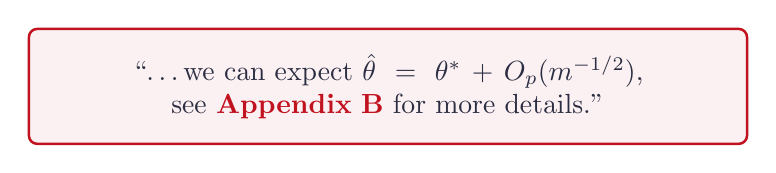
\begin{tikzpicture}
      \node[draw=accent, fill=accent!6, rounded corners=3pt, line width=0.9pt,
            inner sep=9pt, text width=0.7\textwidth, align=center, text=ink] {
        ``\dots we can expect $\hat\theta=\theta^*+O_p(m^{-1/2})$,
        see \hl{Appendix B} for more details.''};
    \end{tikzpicture}\par}
  \vspace{0.9em}

  \onslide<2->{\centering Read it as: the \hl{pre-training error} $\hat\theta-\theta^*$ \emph{shrinks} at rate $1/\sqrt{m}$.\par}
  \vspace{0.3em}
  \onslide<2->{\centering {\footnotesize\mut{(not ``quality grows like $\sqrt m$'' --- the \emph{error} decays like $m^{-1/2}$, so $\hat\theta\to\theta^*$ as $m\to\infty$.)}}\par}
  \vspace{0.7em}

  \onslide<3->{\centering
    \begin{tabular}{ll}
      \hl{$\theta^*$} & the KL-optimal parameter \mut{(best the model can do on the prior)} \\
      \hl{$\hat\theta$} & what pre-training actually returns from $m$ simulated sets \\
    \end{tabular}\par}
  \vspace{0.6em}

  \onslide<3->{\centering {\gd{And yes --- Appendix B \emph{is} exactly the section this points to.}}\par}
\end{frame}

% ===========================================================================
\begin{frame}[t]{Step 1 --- what is pre-training even maximizing?}

  \onslide<1->{\centering
    An \hl{objective} $=$ one number that \emph{grades} a parameter setting $\theta$ \mut{(bigger $=$ better predictions)}.\\
    Pre-training turns the knobs $\theta$ to push this grade as high as it goes. \mut{\footnotesize (like maximizing a test score)}\par}
  \vspace{0.5em}
  \onslide<1->{\centering
    {\footnotesize\mut{The grade here is the \emph{average log-likelihood}: how much probability $q_\theta$ puts on the \emph{correct} label.}}\par}
  \vspace{0.6em}

  \begin{columns}[T]
    \column{0.5\textwidth}
      \onslide<2->{\begin{block}{The grade we \emph{wish} we had}
        \centering $\displaystyle L(\theta)=\mathbb{E}_{\Pi_N}\mathbb{E}_{\Pi}\bigl[\log q_\theta\bigr]$\\[5pt]
        {\footnotesize average over \hl{all possible} datasets the prior can make \mut{(ideal, infinite --- can't compute)}}\\[4pt]
        {\footnotesize its best $\theta=$ \hl{$\theta^*$}}
      \end{block}}
    \column{0.5\textwidth}
      \onslide<3->{\begin{block}{The grade we \emph{can} compute}
        \centering $\displaystyle L_m(\theta)=\frac1m\sum_{j=1}^m \log q_\theta\bigl(\mathcal{D}^{(j)}\bigr)$\\[5pt]
        {\footnotesize average over just the \hl{$m$ datasets we actually simulated}}\\[4pt]
        {\footnotesize its best $\theta=$ \hl{$\hat\theta$} \mut{(what training returns)}}
      \end{block}}
  \end{columns}
  \vspace{0.4em}

  \onslide<4->{\centering
    The question: does maximizing the \hl{computable} $L_m$ land near the maximizer of the \hl{true} $L$?\\
    {\gd{Yes} --- and the gap is the $O_p(m^{-1/2})$. \mut{\footnotesize $L_m$ is an \emph{average of $m$ pieces} --- the ``M-estimator'' setup.}}\par}
\end{frame}

% ===========================================================================
\begin{frame}[t]{Aside --- what is the Central Limit Theorem (CLT)?}

  \onslide<1->{\centering
    Take many \hl{independent} random measurements and \hl{average} them. The CLT says:\par}
  \vspace{0.5em}
  \onslide<1->{\centering
    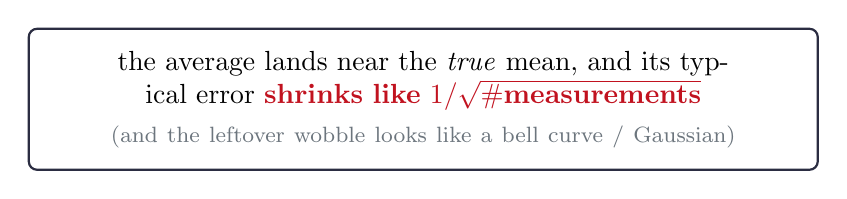
\begin{tikzpicture}
      \node[draw=ink, rounded corners=3pt, line width=0.8pt, inner sep=8pt,
            text width=0.78\textwidth, align=center] {
        the average lands near the \emph{true} mean, and its typical error
        \hl{shrinks like $1/\sqrt{\#\text{measurements}}$}\\[2pt]
        \mut{\footnotesize (and the leftover wobble looks like a bell curve / Gaussian)}};
    \end{tikzpicture}\par}
  \vspace{0.7em}

  \begin{columns}[T]
    \column{0.52\textwidth}
      \onslide<2->{\centering \textbf{Poll analogy}\\[4pt]
        {\footnotesize Ask $m$ random people $\to$ your poll \% is off by $\approx 1/\sqrt m$.\\[3pt]
         \hl{$4\times$ the people $\Rightarrow$ half the error.}}\par}
    \column{0.48\textwidth}
      \onslide<3->{\centering \textbf{the bell narrows as $m\uparrow$}\\[4pt]
      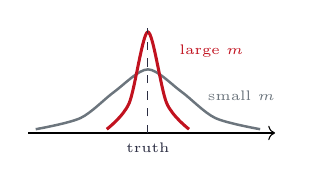
\begin{tikzpicture}[scale=0.95]
        \draw[->] (-0.1,0) -- (3.2,0);
        \draw[muted, line width=0.9pt] plot[smooth]
          coordinates {(0,0.05)(0.6,0.2)(1.05,0.55)(1.5,0.85)(1.95,0.55)(2.4,0.2)(3,0.05)};
        \draw[accent, line width=1.1pt] plot[smooth]
          coordinates {(0.95,0.05)(1.25,0.4)(1.5,1.35)(1.75,0.4)(2.05,0.05)};
        \draw[dashed, ink] (1.5,0) -- (1.5,1.4);
        \node[font=\tiny, muted] at (2.75,0.5) {small $m$};
        \node[font=\tiny, accent] at (2.35,1.1) {large $m$};
        \node[font=\tiny, ink, below] at (1.5,0) {truth};
      \end{tikzpicture}}
  \end{columns}
  \vspace{0.5em}

  \onslide<3->{\centering
    {\gd{Our $L_m$ is exactly such an average}} (over $m$ datasets) --- so its error, and $\hat\theta$'s, shrink like $1/\sqrt m$.\par}
\end{frame}

% ===========================================================================
\begin{frame}[t]{Why $\sqrt{m}$: a noisy hill has a slightly-shifted peak}

  \onslide<1->{\centering
    Picture each objective as a \hl{hill} over $\theta$; the best $\theta$ is the \hl{peak} (slope flat).
    $L_m$ is a \hl{noisy copy} of the true hill $L$ $\Rightarrow$ its peak $\hat\theta$ sits just off $\theta^*$.\par}
  \vspace{0.2em}

  \onslide<1->{\centering
  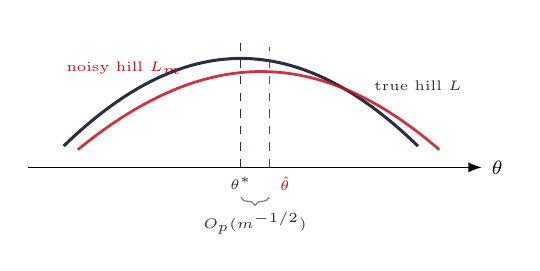
\begin{tikzpicture}[>=Latex, font=\scriptsize, scale=0.9]
    \draw[->] (0,0) -- (6.4,0) node[right]{$\theta$};
    \draw[ink, line width=1.1pt] (0.5,0.3) .. controls (2.2,1.95) and (3.8,1.95) .. (5.5,0.3);
    \node[ink, font=\tiny] at (5.5,1.15) {true hill $L$};
    \draw[accent, line width=1.0pt, opacity=0.85] (0.7,0.25) .. controls (2.5,1.72) and (4.1,1.72) .. (5.8,0.25);
    \node[accent, font=\tiny] at (1.35,1.4) {noisy hill $L_m$};
    \draw[dashed, ink] (3.0,0) -- (3.0,1.85); \node[ink, font=\tiny, below] at (3.0,0) {$\theta^*$};
    \draw[dashed, accent] (3.4,0) -- (3.4,1.7); \node[accent, font=\tiny, below] at (3.62,0) {$\hat\theta$};
    \draw[decorate, decoration={brace, amplitude=3pt, mirror}, muted]
      (3.0,-0.42) -- (3.4,-0.42) node[midway, below=2pt, font=\tiny, text=ink] {$O_p(m^{-1/2})$};
  \end{tikzpicture}}
  \vspace{0.2em}

  \onslide<2->{\textbf{1.} At $\theta^*$ the true slope is $0$ --- but the \hl{noisy} slope of $L_m$ isn't quite $0$.\par}
  \onslide<3->{\textbf{2.} That leftover slope is an \hl{average of $m$ independent pieces} $\Rightarrow$ by the \hl{CLT}, $\approx 1/\sqrt m$ in size.\par}
  \onslide<4->{\textbf{3.} A small slope-error shifts the peak proportionally \mut{(less if the hill is sharply curved)} $\Rightarrow$ \gd{$\hat\theta-\theta^*\approx 1/\sqrt m$}. \mut{\footnotesize (slope $=$ gradient, curvature $=$ Hessian.)}\par}
\end{frame}

% ===========================================================================
\begin{frame}[t]{Appendix B, Thm B.1 --- the parameter}

  \onslide<1->{\centering
    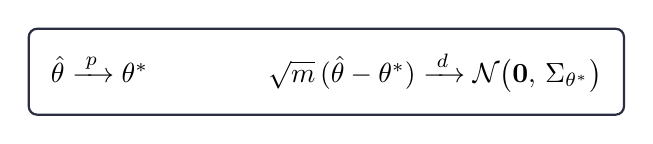
\begin{tikzpicture}
      \node[draw=ink, rounded corners=3pt, line width=0.8pt, inner sep=8pt, align=center] {
        $\hat\theta\xrightarrow{\;p\;}\theta^*$
        \qquad\qquad
        $\sqrt{m}\,(\hat\theta-\theta^*)\xrightarrow{\;d\;}\mathcal{N}\bigl(\mathbf{0},\,\Sigma_{\theta^*}\bigr)$};
    \end{tikzpicture}\par}
  \vspace{0.7em}

  \onslide<2->{\centering The covariance is a \hl{``sandwich''}: \;$\Sigma_{\theta^*}=\underbrace{I_{\theta^*}^{-1}}_{\text{bread}}\,\underbrace{V_{\theta^*}}_{\text{filling}}\,\underbrace{I_{\theta^*}^{-1}}_{\text{bread}}$\par}
  \vspace{0.5em}

  \begin{columns}[T]
    \column{0.5\textwidth}
      \onslide<2->{\centering \hl{$I_{\theta^*}=\mathbb{E}[\nabla^2\log q_{\theta^*}]$}\\ {\footnotesize\mut{curvature --- how sharply peaked the optimum is}}\par}
    \column{0.5\textwidth}
      \onslide<2->{\centering \hl{$V_{\theta^*}=\mathbb{E}[\nabla\log q_{\theta^*}\nabla^{\!\top}\!\log q_{\theta^*}]$}\\ {\footnotesize\mut{score covariance --- the CLT variance}}\par}
  \end{columns}
  \vspace{0.6em}

  \onslide<3->{\centering
    {\footnotesize\mut{Why the sandwich (not plain inverse-Fisher)? The PFN is \hl{misspecified} ($q_\theta\neq\pi$), so $V\neq-I$.}}\\[2pt]
    {\footnotesize\mut{Proof $=$ a citation: van der Vaart \& Wellner (1996), Cor.\ 3.2.3 \& Ex.\ 3.2.12.}}\par}
\end{frame}

% ===========================================================================
\begin{frame}[t]{Appendix B, Thm B.2 --- from $\hat\theta$ to the prediction}

  \onslide<1->{\centering
    Push the rate from the parameter onto the actual output $q_{\hat\theta}$ \mut{(continuous mapping $+$ delta method)}:\par}
  \vspace{0.6em}

  \begin{columns}[T]
    \column{0.52\textwidth}
      \onslide<2->{\centering
        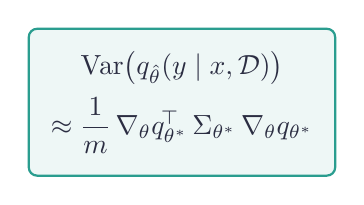
\begin{tikzpicture}
          \node[draw=good, fill=good!8, rounded corners=3pt, line width=0.8pt, inner sep=8pt, align=center, text=ink] {
            $\operatorname{Var}\bigl(q_{\hat\theta}(y\mid x,\mathcal{D})\bigr)$\\[4pt]
            $\approx\dfrac{1}{m}\,\nabla_\theta q_{\theta^*}^{\!\top}\,\Sigma_{\theta^*}\,\nabla_\theta q_{\theta^*}$};
        \end{tikzpicture}\par}
    \column{0.48\textwidth}
      \onslide<3->{\centering \textbf{\footnotesize decays like $1/m$}\\[2pt]
      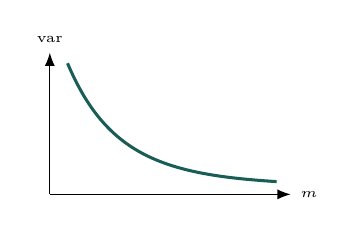
\begin{tikzpicture}[>=Latex, scale=0.9]
        \draw[->] (0,0) -- (3.4,0) node[right, font=\tiny]{$m$};
        \draw[->] (0,0) -- (0,2.0) node[above, font=\tiny]{var};
        \draw[good!60!black, line width=1.1pt] (0.25,1.85) .. controls (0.8,0.55) and (1.6,0.28) .. (3.2,0.18);
      \end{tikzpicture}}
  \end{columns}
  \vspace{0.7em}

  \onslide<4->{\centering
    Variance scales with \hl{(a)} how tightly $\hat\theta$ is pinned ($\Sigma_{\theta^*}$) and \hl{(b)} how sensitive the output is to $\theta$ ($\nabla_\theta q$).\par}
  \vspace{0.2em}
  \onslide<4->{\centering {\gd{$\Rightarrow$ more complex models need a larger $m$.}}\par}
\end{frame}

% ===========================================================================
\begin{frame}[t]{Where this sits: the four knobs of Section 4}

  \onslide<1->{\centering The PFN approximation depends on \hl{four} factors:\par}
  \vspace{0.7em}

  \onslide<1->{\centering
  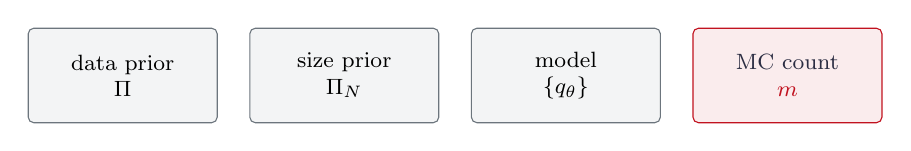
\begin{tikzpicture}[font=\footnotesize, knob/.style={draw=muted, rounded corners=2pt, fill=muted!8, minimum width=24mm, minimum height=12mm, align=center}]
    \node[knob] (pi) {data prior\\ $\Pi$};
    \node[knob, right=4mm of pi] (pin) {size prior\\ $\Pi_N$};
    \node[knob, right=4mm of pin] (q) {model\\ $\{q_\theta\}$};
    \node[knob, right=4mm of q, draw=accent, fill=accent!8, text=ink] (m) {MC count\\ \hl{$m$}};
  \end{tikzpicture}}
  \vspace{0.9em}

  \onslide<2->{\centering
    \hl{$m$} $\to$ Appendix B $\to$ $O_p(m^{-1/2})$: a \emph{classical, off-the-shelf} estimation rate.\par}
  \vspace{0.4em}

  \onslide<3->{\centering
    {\footnotesize\mut{The paper calls this axis ``\emph{rather uneventful}'': it is \hl{orthogonal} to the in-context story (which is driven by $n$, not $m$).}}\par}
  \vspace{0.3em}
  \onslide<3->{\centering
    {\footnotesize\mut{$\Pi_N$ (size of each set) is the ``complexity regularizer''; \hl{$m$ (how many sets)} is this $\sqrt m$ rate --- two separate knobs.}}\par}
\end{frame}

% ===========================================================================
\begin{frame}[standout]
  $\hat\theta$ is just an M-estimator over $m$ iid simulated sets.\\[6pt]
  So it is $\sqrt{m}$-consistent (Appendix B) --- the \emph{boring} axis,\\
  orthogonal to in-context learning in $n$.
\end{frame}

\end{document}
